% !TeX program = xelatex
\documentclass{alex_bericht}

\usepackage{ifxetex,ifluatex}
\usepackage{etoolbox}
\usepackage[svgnames]{xcolor}

\usepackage{tikz}

\usepackage{framed}

% conditional for xetex or luatex
\newif\ifxetexorluatex
\ifxetex
\xetexorluatextrue
\else
\ifluatex
\xetexorluatextrue
\else
\xetexorluatexfalse
\fi
\fi
%
\ifxetexorluatex%
\usepackage{fontspec}
\usepackage{libertine} % or use \setmainfont to choose any font on your system
\newfontfamily\quotefont[Ligatures=TeX]{Linux Libertine O} % selects Libertine as the quote font
\else
\usepackage[utf8]{inputenc}
\usepackage[T1]{fontenc}
\usepackage{libertine} % or any other font package
\newcommand*\quotefont{\fontfamily{LinuxLibertineT-LF}} % selects Libertine as the quote font
\fi

\newcommand*\quotesize{60} % if quote size changes, need a way to make shifts relative
% Make commands for the quotes
\newcommand*{\openquote}
{\tikz[remember picture,overlay,xshift=-4ex,yshift=-2.5ex]
	\node (OQ) {\quotefont\fontsize{\quotesize}{\quotesize}\selectfont``};\kern0pt}

\newcommand*{\closequote}[1]
{\tikz[remember picture,overlay,xshift=4ex,yshift={#1}]
	\node (CQ) {\quotefont\fontsize{\quotesize}{\quotesize}\selectfont''};}

% select a colour for the shading
\colorlet{shadecolor}{white}

\newcommand*\shadedauthorformat{\emph} % define format for the author argument

% Now a command to allow left, right and centre alignment of the author
\newcommand*\authoralign[1]{%
	\if#1l
	\def\authorfill{}\def\quotefill{\hfill}
	\else
	\if#1r
	\def\authorfill{\hfill}\def\quotefill{}
	\else
	\if#1c
	\gdef\authorfill{\hfill}\def\quotefill{\hfill}
	\else\typeout{Invalid option}
	\fi
	\fi
	\fi}
% wrap everything in its own environment which takes one argument (author) and one optional argument
% specifying the alignment [l, r or c]
%
\newenvironment{shadequote}[2][l]%
{\authoralign{#1}
	\ifblank{#2}
	{\def\shadequoteauthor{}\def\yshift{-2ex}\def\quotefill{\hfill}}
	{\def\shadequoteauthor{\par\authorfill\shadedauthorformat{#2}}\def\yshift{2ex}}
	\begin{snugshade}\begin{quote}\openquote}
		{\shadequoteauthor\quotefill\closequote{\yshift}\end{quote}\end{snugshade}}


\begin{document}	
%Seiten ohne Kopf- und Fußzeile sowie Seitenzahl
\pagenumbering{Roman}
\def\settitle{Essay on Edwin Hubble's paper on the expansion of the Universe}
% !TeX root = Bericht.tex
% !TeX spellcheck = de_AT
\thispagestyle{empty}
\titlehead{
\includegraphics[width=5cm]{logo.jpg}}
\title{Über das Aussehen von relativistisch ausdehnende Radioquellen}
\author{Alexander Helbok\thanks{\href{alexander.helbok@student.uibk.ac.at}{alexander.helbok@student.uibk.ac.at}}}
\date{\today}
\maketitle
\vfill 



%Inhaltsverzeichnis
\hypersetup{linkcolor=black}
\clearpage
\tableofcontents

\hypersetup{linkcolor=MyBlue}

%\cleardoubleoddpage

\pagenumbering{arabic}
% !TeX root = Bericht.tex
% !TeX spellcheck = de_DE
\section{Einleitung}
\label{sec:einleitung}
In 60 Jahren kann sich das physikalische Weltbild stark verändern. Vor allem wenn man an die erste Hälfte des 20. Jahrhunder denkt, wo ein ganzer Teilbereich mit der Quantenmechanik neu aufgestellt wurde. Dennoch waren Physiker sich der Implikationen von Einsteins  Relativitätstheorie auch nach 60 Jahren noch nicht ganz bewusst. Wie die Welt bei relativistischen Geschwindigkeiten aussieht, kann man nur anhand mathematischer Formeln erahnen, so kontraintuitiv sind die Konzepte der SRT.

So geschah es, dass 1966 (61 Jahre nach Veröffentlichung der speziellen Relativitätstheorie), die starken Helligkeitsschwankungen von entfernten Radioquellen durch ein simples geometrisches Argument erklärt werden konnten. 
Das geometrische Argument trägt aber auch ein scheinbares Paradoxon mit sich, und zwar sich mit Übberlichtgeschwindigket ausdehnende Körper.

% !TeX root = Bericht.tex
% !TeX spellcheck = en_US
\section{paper review}\label{theorie}
I will start by giving a brief overview of the measurement setup and collected data before diving into the analysis that Edwin Hubble performed to reach his results. Lastly I will go through Hubble's interpretation of his finding and compare it to today's knowledge. 

Edwin Hubble worked at the Mount Wilson Observatory in California, which hosts the \( 100 \unit{in} \) Hooker telescope, the largest telescope in the world from \( 1917 \) to \( 1949 \). The telescope's large aperture provided unprecedented resolution and light-gathering power, allowing astronomers to observe faint nebulae and identify individual Cepheid variable stars within them. Additionally, photographic plates were used to record both images and spectra, which are essential when making quantitative comparisons.

With these technological advancements and building upon the work of fellow astronomers, Hubble combined distance measurements with existing velocity data to make his groundbreaking discovery. Vesto Melvin Slipher used Doppler spectroscopy to measure and publish radial velocities of many nebulae \autocite{slipher1915spectrographic}. Even though Hubble never mentions where the velocity measurements come from in his 1929 paper, he does so in other publications so it can be assumed that the same is true here. As for distances, Hubble used different methods to estimate them. For nearby nebulae Hubble identified Cepheid variable stars and used the period-luminosity relation to calculate the distance. Due an incorrect zero point calibration Hubble systematically underestimated the distances, which will become apparent later. For more distant nebulae Edwin Hubble used the fact that there is an upper limit for stellar luminosity (also known as the Eddington limit). Using the apparent magnitude of the brightest stars and assuming their absolute magnitude to be close to the limit he calculated their distance (essentially treating the brightest observable stars as standard candles). The last four nebulae were not identified to lie in the Virgo cluster, whose distance can be estimated using the statistical distribution of nebular luminosities. The original plot showing the collected data is shown in \autoref{fig:hubble}, with annotations to break the content down. One can clearly see the different regimes of distance estimation, with the closest ones being the Cepheids, central datapoints are nebulae in which very bright stars can be singled out and used as standard candles and the most distant being the four nebulae in the Virgo cluster.

Additionally the data was binned and is shown as hollow points. Unfortunately the details of the binning process are not mentioned. Lastly, 22 nebulae for which individual distance estimates were unsuccessful were condensed into the black cross representing the mean velocity and mean distance. 

\begin{figure}[H]
	\begin{tikzpicture}
		\begin{scope}[xshift=1.5cm]
			\node[anchor=south west,inner sep=0] (image) at (0,0) {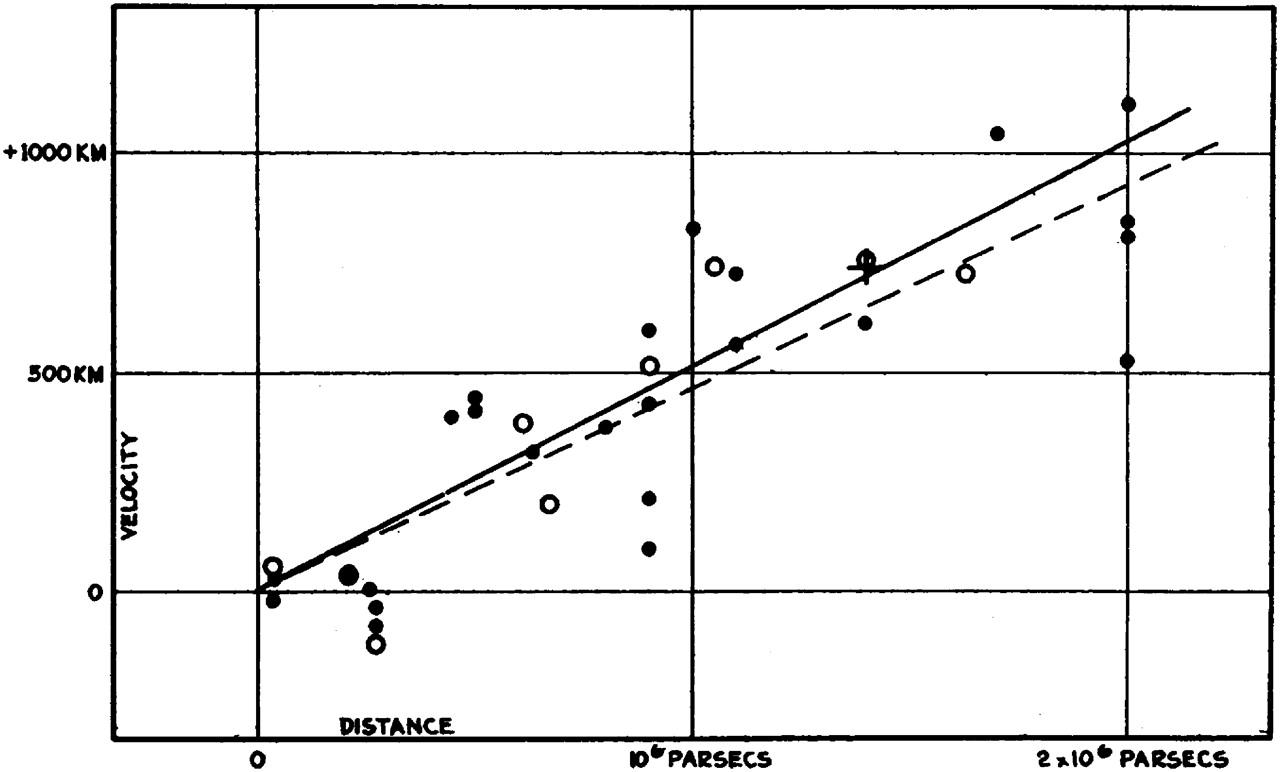
\includegraphics[width=\textwidth]{HubbleLaw}};
			\begin{scope}[x={(image.south east)},y={(image.north west)}]
				\fill[Gray, opacity=0.3, rounded corners] (0.205, 0.665) rectangle (0.5, 0.97);
				\draw[MyOrange,ultra thick,rounded corners] (0.2,0.15) rectangle (0.31,0.3);
				\draw[MyOrange,ultra thick,rounded corners] (0.335,0.43) rectangle (0.37,0.49);
				
				\draw[rotate around={-60:(0.575,0.55)},MyBlue, ultra thick] (0.575,0.55) ellipse (40pt and 95pt);
				
				
				\draw[MyRed,ultra thick,rounded corners] (0.86,0.5) rectangle (0.9,0.9);
				
%				Legend
				\begin{scope}[shift={(-0.48, 0.6)}]							
					\draw[MyOrange,ultra thick,rounded corners] (0.7,0.3) rectangle (0.73,0.35) node [black, right, yshift=-0.18cm] {Cepheids};
					\draw[MyBlue,ultra thick,rounded corners] (0.7,0.22) rectangle (0.73,0.27) node [black, right, yshift=-0.18cm] {standard candles};
					\draw[MyRed,ultra thick,rounded corners] (0.7,0.14) rectangle (0.73,0.19) node [black, right, yshift=-0.18cm] {Virgo};
					\draw[ultra thick, line cap=round] (0.7, 0.1) -- (0.73, 0.1) node [right] {fit};
				\end{scope}
				
				\fill[Gray, opacity=0.3, rounded corners] (0.69, 0.25) rectangle (0.875, 0.39);
%				Legend
				\begin{scope}[shift={(0, 0.12)}]
					\draw[line width=1.25pt] (0.715,0.24) circle (2 pt) node [right, xshift=0.18cm] {binned data};
					\draw[ultra thick, line cap=round, dashed] (0.7, 0.16) -- (0.73, 0.16) node [right] {fit};
				\end{scope}
				
				\fill[Gray, opacity=0.3, rounded corners] (0.69, 0.15) rectangle (0.875, 0.22);				
				\begin{scope}[shift={(0, -0.055)}]
					\draw[line width=1.75pt, line cap=round] (0.7, 0.24) -- (0.73, 0.24) node [right, xshift=0.05cm] {mean data};
					\draw[line width=1.75pt, line cap=round] (0.715, 0.22) -- (0.715, 0.26);
				\end{scope}
			\end{scope}
		\end{scope}
	\end{tikzpicture}
	\caption{The original image from \autocite{Hubble1929} showing the velocity of various nebulae against their calculated distance. The image has been broken down into three layers visualizing different parts of the data analysis. 1) Black dots stand for individual datapoints and are color coded to hint at the method used for determining the distance. The black solid line represents the linear regression to these datapoints. 2) Hollow white circles represent binned datapoints. How the binning was performed is unknown. The dashed black line was fitted to the binned data. 3) The mean of all datapoints was computed and is shown as black cross.}
	\label{fig:hubble}
\end{figure}

A linear function was fitted once to all individual datapoints (solid line) and once to the binned data (dashed line) with fitted slopes of 
\begin{equation*}
	K_{\text{all}} = (465 \pm 50) \unit{km/s/Mpc} \qquad\text{and}\qquad K_{\text{binned}} = (513 \pm 60) \unit{km/s/Mpc}.
\end{equation*}

How the regression was performed and the nature of the given uncertainties is not included in the paper. Comparing these values to today's value of around \( H_0 \approx 70 \unit{km/s/Mpc} \) \autocite{Di_Valentino_2021, kamionkowski2023hubble} (we actually get inconsistent results) one can see that the slope is larger by a factor of 7. The paper has been thoroughly analyzed by many astronomers and the mistakes Hubble made were reconstructed \autocite{blunder}. First the Cepheid period-luminosity relation was off by around \( 1.5 \unit{mag} \). Furthermore the Hooker telescope did not map the brightness of objects linearly onto the photographic plate, resulting in an additional error of estimated \( 0.6 \unit{mag} \). Lastly, for the more distant galaxies Hubble was unable to distinguish bright stars from HII regions. He mistakenly used these regions (which are around 2 magnitudes brighter than the brightest stars) to underestimate the distance to the Virgo cluster for example. The combination of these effects led to a result that is roughly 7 times larger than the range we are dealing with today.

Finally, let's come to the interpretation of the aforementioned results. 

\begin{shadequote}[r]{Edwin Hubble \autocite{Hubble1929}}
	The results establish a roughly linear relation between velocities and distances among nebulae ...
\end{shadequote}
This statement is correct in many ways. A linear relation can be hinted at in the data and Hubble is right in being a bit cautious and calling it a \blockquote{roughly} linear relation. From the wrong Cepheid calibration to using statistical arguments for distance estimation, a quantitative discussion need a deeper understanding of the physics at play (as can be seen in the deviation from the now accepted value for \( H_0 \)). Nevertheless, Hubble's approach to measuring distances is sound (using standard candles) and he correctly identified the linear trend so credit has to be given where credit is due. 


\begin{shadequote}[r]{Edwin Hubble \autocite{Hubble1929}}
	New data to be expected in the near future may modify the significance of the present investigation or, if confirmatory, will lead to a solution having many times the weight.
\end{shadequote}
This is absolutely right. Many experiments have been conducted up until today and all confirm that distant object are receding away from us faster and faster. The cosmic expansion has not remained constant in the past, it is actually accelerating (a Nobel Prize was awarded for this discovery). Mapping the evolution of the Hubble parameter leads crucial insight into the evolution and composition of the universe.  There are two different ways for determining \( H_0 \). One is a bottom-up approach in which we \blockquote{climb the distance ladder} and determine \( H_0 \) from the the slope of the curve and a top-down approach in which the parameter is calculated from the state of the early universe (via the cosmic background radiation). The two methods yield statistically inconsistent values for \( H_0 \) the reason of which remains a major question in the field of astrophysics (also known as \blockquote{crisis in cosmology} or \blockquote{Hubble tension}).

\begin{shadequote}[r]{Edwin Hubble \autocite{Hubble1929}}
	The outstanding feature, however, is the possibility that the velocity-distance relation may represent the de Sitter effect, ...
\end{shadequote}

In the last chapter of the paper Edwin Hubble blunders and tries to connect the data to the de Sitter effect. The de Sitter universe is a model of a static universe filled with dark energy and was created by Willem de Sitter. The feature of this model Hubble refers to is that time runs slower for more distant objects, making them appear redshifted. This idea was disregarded by de Sitter himself \autocite{deSitter1930proceedings} as the de Sitter model does not specify in any way how matter is distributed along different geodesics and a linear velocity-distance relation is only valid for certain matter distributions \autocite{deSitter}. After the publication of Hubble's paper the physics community became aware of the works of Friedmann and Lema\^{i}tre, which developed solutions to the equations of general relativity predicting an expanding universe and a linear velocity-distance relation. 

As a short sidenote I would like to entertain the question whether Hubble actually was the first person to notice the linear relation and calculate its slope. As a matter of fact, he was not. Two physicists beat him to it but went largely unnoticed due to a combination of publishing in obscure journals and using different ways to calculate distances introducing even larger errors. The first person to note this connection was Lundmark in 1925 \autocite{lundmark1925motions}, treating the nebulae as standard rulers (e.g. using the apparent size instead of apparent brightness to calculate distances). He found a quadratic relation and rejected a linear function which he also tried out. Two years later Lema\^{i}tre used data published by Hubble in 1924 \autocite{lemaitre1927univers}. Instead of using the brightest stars in galaxies as standard candles Lema\^{i}tre used the apparent brightness of galaxies combined with Hubble's conjecture of being able to extrapolate the mean luminosity of nearby galaxies to more distant objects. This turns out to be wrong since the sample of distant nebulae was biased towards more bright ones, as they are more likely to be picked up by the telescope (this is also known as Malmquist bias). Hubble is therefore credited with discovering the linear relation between velocity and distance. 




















% !TeX root = Bericht.tex
% !TeX spellcheck = en_US
\section{personal outlook}
Lastly, I would like to give a brief outlook onto my further university studies. I just finished my first semester in the physics master program and so far I quite enjoy the freedom of choice regarding the courses. It not only allows me but also motivates me to explore my interests in various fields of physics. So far I have attended a healthy mix of experimental, data analysis and theory courses and I have found out one thing: I am not a theorist. Although I enjoy the concepts of theoretical physics the maths involved is not my thing. I have always been quite fond of (extragalactic) astrophysics as the night sky is just marvelous to look at and hosts many unanswered questions. This led me to write my high school thesis on Quasars and observable phenomena (Jets, apparent superluminal velocities, gravitational lensing). During my undergraduate degree, I really valued the lab courses as they allowed me to apply my passion for data analysis in practice, offering a welcome balance to the otherwise dry and theoretical curriculum.

For this reason I chose to write my bachelor thesis in the institute of experimental physics under the supervision of Prof. Kirchmair. In my thesis I combined measurements from the lab with electromagnetic simulations to extract the origin and relative magnitude of losses in microwave resonators. This is as the uncovers the connection between manufacturing defects and coherence times in superconducting circuits. Even though the involved physics was not the most interesting, I got to manufacture the samples in the cleanroom, perform the measurements in the lab, set the simulations up and lastly analyze and compare the collected data. As a whole it was a really enjoyable and motivating experience as the tasks to perform were quite diverse and I had the feeling the work I was doing is of actual interest to the research group. For this reason I will probably also write my master thesis in the same research group as no other group (to my knowledge) offers the same level of diversity.

Next semester, I plan to attend a mix of different courses with a slight bias towards quantum engineering, as this knowledge will help me in my thesis. Looking further as the masters degree I could see myself doing a PhD and stay in academia after that as the idea of research and education is appealing to me. 

%\input{05_Ergebnisse}

%\input{06_Diskussion}

%%Literaturverzeichnis
\printbibliography

\end{document}
